% *******************************************************************************
% * Copyright (c) 2007 by Elexis
% * All rights reserved. This document and the accompanying materials
% * are made available under the terms of the Eclipse Public License v1.0
% * which accompanies this distribution, and is available at
% * http://www.eclipse.org/legal/epl-v10.html
% *
% * Contributors:
% *    G. Weirich - initial implementation
% *
% *  $Id: settings.tex 2563 2007-06-23 04:56:40Z rgw_ch $
% *******************************************************************************
%
% !Mode:: "TeX:UTF-8" (encoding info for WinEdt)

\label{settings}
Die Einstellungen sind alle im selben Dialog zusammengefasst, welcher unter
\textsc{Datei-Einstellungen} erreicht werden kann (Abb. \ref{fig:settingsmain}). 
%\usepackage{graphics} is needed for \includegraphics
\begin{figure}[htp]
\begin{center}
  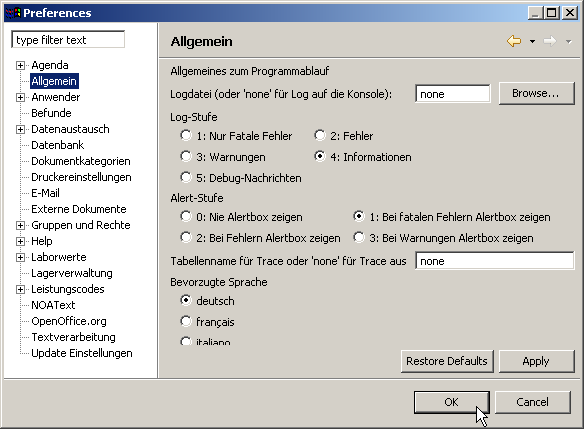
\includegraphics[width=0.6\textwidth]{images/settingsmain}
  \caption{Einstellungs-Dialog}
  \label{fig:settingsmain}
\end{center}
\end{figure}


Wie üblich in Elexis ist der genaue Inhalt dieses Dialogs davon abhängig,
welche Plugins installiert sind. Mit den Reitern auf der linken Seite wählt man
einen Bereich aus, für den man EInstellungen ändern möchte. Wir gehen hier auf
diejenigen Seiten ein, die zur Grundausstattung von Elexis gehören. Grundsätzlich
sollten alle Einstellungen \glqq Ab Werk\grqq{}vernünftige Grundeinstellungen
aufweisen, so dass es zunächst nicht nötig ist, hier etwas zu ändern. Sie
brauchen daher dieses Kapitel auch nicht unbedingt weiterzulesen.

\section{Allgemein}
Auf dieser Seite werden allgemeine Einstellungen für den Programmablauf
definiert. Es sind dies:
\subsection{Einstellungen zum Log}
Das \glqq Log\grqq{} ist das Logbuch eines Programmes. Hier werden verschiedene
Information zum Programmablauf gespeichert, welche z.B. bei der Fehlersuche
nützlich sein können.
\begin{itemize}
  \item Logdatei: Der Ort, an den die Log-Informationen gespeichert werden. Die
  sollte normalerweis eeine Datei \glqq elexis.log\grqq{} in Ihrem
  Datenverzeichnis sein. Der Wert \glqq none\grqq{} ist nur sinnvoll, wenn Sie
  Elexis aus einer Entwicklungsumgebung heraus starten.
  \item Log-Stufe: Wieviele Meldungen ausgegeben werden sollen. Auf Stufe 1
  werden nur die allerschlimmsten Fehler, die einen Programmabbruch erzwingen,
  ausgegeben. Auf Stufe 5 werden sehr viele Meldungen, die nur in speziellenj
  Fällen sinnvoll sind, ins Log geschrieben. Wir empfehlen für den Normalbetrieb
  Stufe 2 oder 3.
  \item Alert-Stufe: Meldungen, die den entsprechenden Schweregrad haben, werden
  nicht nur ins Log geschrieben, sondern gleich am Bildschirm angezeigt.
  Achtung: Wenn Sie hier eine zu hohe Stufe angeben, werden Sie ständig durch
  aufpoppende Meldungsboxen irritiert werden. Wir empfehlen Stufe 1.
  \item Tabellenname für Trace: Trace bedeutet, dass alle Aktionen in einer
  speziellen Tabelle aufgezeichnet werden. Es lässt sich damit später
  nachvollziehen, von welcher Arbeitsstation aus zu welchem Zeitpunkt welche
  Aktion mit Elexis durchgeführt wurde. Dies erlaubt eine sehr genaue Kontrolle
  der Vorgänge, kostet aber natürlich Arbeitsgeschwindigkeit und Speicherplatz.
  Wir empfehlen im Normalfall die Einstellung \glqq none\grqq{}.
  \item Bevorzugte Sprache: Diese Einstellung definiert nicht, welche
  Sprachversion von Elexis ausgeführt wird (Das wird anhand der
  Betriebssystemeinstellungen und ggf. Startparameter entschieden), sondern
  vielmehr, welche Tarmed- und ICD-Versionen etc. importiert werden.
  \item Speicherdauer im Cache: Dies ist eine sehr technische Einstellung. Es
  geht darum, wie lange aus der Datenbank gelesene Objekte gültig bleiben
  sollen, bevor sie erneut gelesen werden. Wenn
  viele Arbeitsstationen im Netz sind, geben Sie hier besser kürzere Zeiten an
  (z.B. 5 Sekunden), wenn Sie von zuhause über eine langsame Internet-Verbindung
  auf Elexis zugreifen, eher eine längere Zeit (z.B. 300 Sekunden).
  \item Aktualisierungsintervall: Nach welcher Zeitspanne soll Elexis jeweils
  seine Views aktualisieren. Wenn beispielsweise die MPA einen Patienten der
  Agenda auf \glqq eingetroffen\grqq{} setzt, dann dauert es maximal soviele
  Sekunden, bis diese Statusänderung auf Ihrem Bildschirm sichtbar ist. Wenn Sie
  zu kurze Zeiten angeben, wird die Netzwerkbelastung unnötig hoch.
\end{itemize}
\section{Anwender}
In diesem Zweig der Einstellungen sind anwenderspezifische Einstellungen
untergebracht. Wenn Sie einheitliche Einstellungen möchten, können Sie auch einen
Einstellungssatz unter einem frei wählbaren Namen speichern und von einem
anderen Anwenderaccount oder Abreitsstation aus wieder unter diesem Namen laden.

Die Buttons \glqq Einstellungen laden von\ldots\grqq{} bzw. \glqq Einstellungen
speichern nach\ldots\grqq{} betreffen hierbei die anwenderspetifischen
Einstellungen(im Wesentlichen alles was im Zweig \textsc{Anwender} der
Einstellungen vorhanden ist), während die Buttons \glqq
Arbeitsplatzeinstellungen \ldots\grqq{} die auf der lokalen Station
gespeicherten Perspektivenlayouts betreffen. 
